\section{Scalability Bug}
\label{sec-sck-observe}

% example
Scalability bugs in distributed systems is not a well understood problem.
To begin our work on combating scalability bugs, we start by conducting a study
to understand their nature and emphasize how critical they are.
%
We perform a study of \totAll scalability bugs reported from the deployments
of popular large-scale systems such as
Hadoop,
HBase,
HDFS,
Cassandra,
Couchbase,
Riak, and
Voldemort.
%
From the study, we observed many challenges in finding, reproducing, and
debugging scalability bugs. For example, let us consider a bug in Cassandra, a
highly-scalable peer-to-peer key-value store. If a user decommissions a single
node from a cluster of 50 nodes, the operation can be done smoothly. However, if
the user decommissions a node from a cluster of 200 nodes, the protocol that
re-calculate the key-range partitions (which nodes should own which key ranges)
becomes CPU intensive as the calculation has an $O(N^3)$ complexity where $N$ is
the number of nodes.  This combined with the gossiping and failure detection
logic leads to a scalability bug that makes the cluster unstable (many live
nodes are declared as dead, making some data not reachable by the users). We
give a full detail of the Cassandra bug in Section \ref{mot-bug}.

%
As in the example above, bug symptoms sometimes surface only in large deployment
scales (\eg, $N$$>$100 nodes), hence small/medium-scale testing is not enough.
Yet, not all developers have large test budgets, and even when they do,
debugging on hundreds of nodes is time consuming and difficult.
%
Furthermore, protocol algorithms can be scalable in the design sketches, but not
necessarily in the real deployments; there are specific implementation details
whose implications at scale are hard to predict. We discuss more about our
observations on scalability bugs in Section \ref{mot-observe}.

\subsection{A Sample Cassandra Bug}
\label{mot-bug}

\begin{figure}

\centerline{
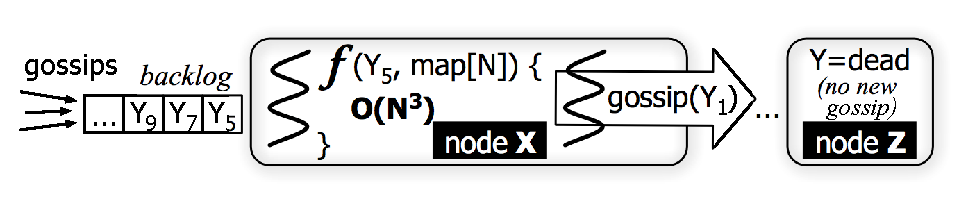
\includegraphics[height=0.8in]{F/cass1.eps}
%\includegraphics[height=0.6in]{F/empty.eps}
}
\vminfive
\mycaption[The problem of gossip-based failure detection in
Cassandra]{fig-cass1}{The problem of gossip-based failure detection in
Cassandra}{}
\vminfive
\end{figure}



We now describe in detail a scalability bug in Cassandra, which we use as a
sample bug.
%
Our journey in understanding scalability bugs began when we observed repeated
``flapping'' problems in large-scale Cassandra deployments (\ie, hundreds of
nodes).
%
Flapping is a cluster instability problem where node's up/down status
continuously flaps.  A ``flap'' is when a node X marks a peer node Y as down
(and soon marks Y as alive again).
%
We rigorously study a series of Cassandra bugs below that surfaced as the code
evolved.

%
%The bug surfaced on a cluster with hundreds of nodes and led to
%``\textit{\textbf{flapping}}'' nodes, a condition where node up/down status
%continuously changes;  tens of thousands of flaps\footnote{A ``\textbf{flap}''
%is when a node X marks a peer node Y as down.}  were observed.

To understand this bug, we need to understand the following protocols.

\begin{enumerate}

\item {\bf Bootstrap:} Each node first creates partition keys (\eg, 32 random
numbers) and gossips this information to peer nodes.
 
\item {\bf Gossip broadcast:} {\em Every second}, each node gossips to one
random node about a list of nodes and partitions it knows (including itself)
and their {\em version} numbers.  Each node also increments its version number
(``I'm still alive'') before gossiping.
 
\item {\bf Gossip processing:} The receiving node then finds any state
(metadata) differences between the two nodes to synchronize their views of the
ring.  Eventually, all nodes know about each other.
 
\item {\bf Failure detection:} {\em Every second}, a failure detection daemon
runs \cite{Lakshman+09-Cassandra}.  Put simply, if a node X has not received a
new gossip about Y {\em from anyone} (Y's version has not changed after some
period of time), X will declare Y dead (a flap).  When X receives a new gossip
about Y, it marks Y alive.

\end{enumerate}

% about the bug
There are two factors that induce the bug. The first is the {\em long latency
of scale-dependent state-update gossip processing during bootstrapping} (``f''
in Figure \ref{fig-cass1}).  While gossip processing is usually fast in a
stable cluster, it is expensive during bootstrapping as the gossips carry many
new state changes about the ring; the state-update processing time is
scale-dependent (\ie, greater than $O(N^3)$); the larger the cluster ($N$), the
larger the ring map, the longer the processing time is.
%
This long latency is caused by {\bf (1)} state-update checkpoint to on-disk
database and {\bf (2)} multi-map cloning and updates.
%
The first one is needed for fast fault tolerance; after a node crashes, it can
reboot fast as it knows the latest view of the ring.
%
The second one is preferred for simplicity; Cassandra clones its \ts{MultiMap}
ring table and applies changes one by one to alleviate long write locks.
%
% in order to prevent a long write lock on the ring table which can block other
% user-facing protocols.

% long
The second factor is the {\em single threaded} implementation of gossip
processing. As shown in Figure \ref{fig-cass1},  this inability to process
multiple gossips/state updates concurrently (for the sake of preventing
concurrency bugs) creates a {\em backlog} of new gossips.  For example, in {\em
every second}, Y tells someone it's alive with increasing version number (\eg,
Y$_7$), but the receiving nodes are still busy processing state changes and
only forward Y's old version number (\eg, Y$_1$).  As Y's new gossip is not
propagated on time,  other nodes (\eg, Z) will mark Y as dead.  This happens to
all nodes, not just Y.

% \ca{3831} -------------------------------------------------
The journey starts with Bug \#\ca{3831} \cite{CA-Two}, when a node D is
decommissioned from a cluster ring, D initiates a gossip telling that all other
nodes must rebalance the ring's key-ranges.  This scale-dependent ``pending
key-range calculation'' is CPU intensive with
%
% $O((n^2)log(n))$   % OLD
$O(MN^3log^3(N))$  % Tanakorn
%
complexity; $M$~is the list of key-range changes in the gossip message.  This
in turn leaves many gossips not propagated on time, creating flapping symptoms
that only appear at scale (at 200+ nodes). The developers
then optimized the code to
%
% $O(nlog(n))$  % OLD
$O(MN^2log^2(N))$ complexity.



% \ca{3881} -------------------------------------------------
Soon afterwards (Bug \#\ca{3881} \cite{CA-Tri}), Cassandra added the concept of
virtual partitions/nodes (\eg, $P$$=$$256$ per physical node).  As an
implication, the fix above did not scale as ``$N$'' becomes $N$$\times$$P$.
%
The bug was fixed with a complete redesign of the pending key-range
calculation, making it
% $O(log(N))$ OLD
$O(MNPlog^2(NP))$.

% \ca{5456} -------------------------------------------------
About a year later (\ca{5456} \cite{CA-Four}), Cassandra code employs
multi-threading between the pending key-range calculation and the gossip
processing with a coarse-grained lock to protect sharing of the ring
table.  Unbeknownst to the developers, at scale, the key-range calculation
can acquire the lock for a long time, causing flapping to reappear again.
The fix clones the ring table for the key-range calculation, to release the
lock early.



% \ca{6127} -------------------------------------------------
Later on (\ca{6127} \cite{CA-One}), a similar bug reappeared.  In the above
cases, the problems appeared when the cluster grows/shrinks gradually.
However, if user bootstrap a large cluster (\eg, 500+ nodes) from
scratch (\ie, all nodes do not know each other, with no established
key ranges),
%
the execution traverses a different code path that
performs a fresh ring-table/key-range construction with
$O(MN^2)$ % KORN
complexity.

% \tl{and there is no existing data stored in   the cluster}), 
% \tl{the offending function becomes the keyrange construction} 
%
% keyrange calculation which clones the ring table (a
% \ts{MultiMap}) becomes very expensive.  
%
% Including the cloning $O(N*P)$, we observed an 
% $O(N^3)$  $O(MN^2)$ % KORN complexity.

% ...............
The story continues on (\ca{6345}, \ca{6409}, \etc).  Fast forward today,
Cassandra developers recently started a new umbrella ticket for discussing
``Gossip 2.0,''  supposedly scalable to 1000+
nodes \cite{Gossip20, Gossip20Mail}.
% ---- 
Similar to Cassandra, other large-scale systems are prone to the same
problem.  So far, we have collected and analyzed \totCass Cassandra, \totCouch
Couchbase, \totHadoop Hadoop, \totHBase HBase, \totHDFS HDFS, \totRiak
Riak, and \totVold Voldemort scalability bugs, all caused user-visible
impacts.
%
This manual mining was arduous because there is no searchable jargon for
``scalability bugs''; we might have missed other bugs.
%

\subsection{Observations}
From all the scalability bugs we studied, we make several important observations.

\begin{enumerate}

\item {\bf What is our focus of scalability bugs?}  
%
We manually determine bug repositories of many popular systems and 
categorize scalability bugs into three sub-classes that relate to
CPU/ processing-time (\totAll bugs), load (50), and data size (35),
respectively.
%
We decided to first focus on CPU/processing-time related ones due to the 
``hidden'' nature of the bugs and the fact that almost all of them can 
only surface at scale.
%
Many load or data size related bugs on the other hand can be reproduced in
smaller scale (\eg, load on $d$ dead nodes will add $d$/$(N$$-$$d)$ load
to every live node) and can be addressed with accurate modeling
\cite{Guo+13-CureIsWorse}.
%
From here on, ``scalability bugs'' implies CPU/processing time related
bugs.

\item {\bf Do they exist in many scalable systems?}  We have collected a
total of \totAll\ bugs~in~many scalable distributed systems
(\totCass~in~Cassandra, \totCouch~in~Couchbase, \totHadoop in Hadoop,
\totHBase~in~HBase, \totHDFS~in~HDFS, \totRiak~in~Riak, and
\totVold~in~Voldemort),
%
reported between 2010 to 2016, with 23 of the bugs appeared in the last 4
years.
%
This is an arduous process due to the lack of searchable jargons for
``scalability bugs''; we might have missed some other bugs.

\item {\bf What are the root causes?}
%
We study the buggy code, patches, and developers' discussions and find
that the majority (38) of the bugs are caused by {\em scale-dependent
loops}, which iterate scale-dependent data structures (\eg, list of
nodes); the rest is about logic bugs (single-function testing suffices).
We break them down to three categories below:
%
(1) Nested CPU-intensive loops (12 bugs);
Section \ref{mot-bug} shows an example.
%
(2) Disk IO loops (20 bugs);  the pattern in similar to
Section \ref{mot-bug} but the nested-loop content is disk IOs.
%
(3) Locking-related loops (8 bugs); they can be in the form of locks
inside scale-dependent loops or vice versa.  Two bugs have multiple
categories.
%
% 18 + 6 (originally)
% 2 is the combination of the last two.
%
These patterns suggest that scalability bugs can be found with program
analysis.



% ---------------------------------------
% tag: ??
\item {\bf Where are they located?}  The bugs are within the user-facing
read/write calls (8 bugs) and operational protocols (33 bugs) such as
%
block report,
bootstrap,
consistency repair,
decommission,
de-replication,
distributed fsck,
heartbeat,
job recovery,
log cleaning,
rebalance, and
region assignment
protocols.

\item {\bf When do they happen?}  User-facing protocols (\eg, read/write)
run ``all the time'' in deployment, hence continuously tested.
%
Operational protocols however are not frequently exercised.  Thus, in a
stable-looking cluster, scalability bugs can linger silently until the
buggy operational protocols are triggered (similar to buggy error handling
\cite{Yuan+14-SimpleTesting}).
%
For the bugs in user-facing calls, we find that 4 of them trigger the bugs
in unique workloads such as large deletions or writes after decommission.
%
The bug reporters (customers) claimed that they observed the bug symptoms
in their large deployments (100-1900 nodes).
%
Our finding here suggests that scalability correctness is not merely about
the user-facing paths.  Distributed systems are full of operational paths
that must be scale-tested as well.


% ---------------------------------------
% tag: imp-??
\item {\bf How do scalability bugs impact users?}
%
As the cluster size grows, the symptoms of scale-dependent loops will
appear: CPU utilization spikes, higher operation latencies due to IO
serialization, or unavailable locks for a long period of time.
Although many of the bugs are in the operational protocols, they
cause {\em cascading}, user-visible impacts.
%
For example, as nodes are incorrectly declared dead (\eg, in Section
\ref{mot-bug}), some data are unreachable.
%
In HDFS, scale-dependent operational activities in the master node cause
the global lock to be less available, hence longer time to
process user's read/write requests.

\item {\bf Why were the bugs not found before?}  Our subjective answers are:
%
first, the workloads and the necessary scales to cover the buggy protocols
are not captured in the unit test; creating a scalable unit test is not
straightforward (\sec\ref{sc-test}).
%
Second, protocols might be scalable in design, but not in practice.
Related to the Cassandra bug (Section \ref{mot-bug}), the failure
detector/gossiper \cite{Hayashibara+04-PhiFailureDetector} was adopted
as it is scalable in design \cite{Lakshman+09-Cassandra}.  However,
the design does not account the gossip processing time during
bootstrap/cluster-changes, which can be long, and the subsequent
backlogs.  To fix the bug, the developers tried to ``do the [simple]
math'' \cite{CA-One} but failed.  Specific implementation choices such
as overloading gossips with many other purposes (\eg, announcing
boot/rebalance changes) deviate from the original design sketch.



% -------------------------------------------
\item {\bf Are scalability bugs easy to debug and fix?}
%
The scalability bugs we studied took around 1 month to fix on average
with tens of back-and-forth discussions.
% 6 to 157 days to fix 
One factor of delayed fixes is the lack of budget for large test clusters
(admitted by the developers; \sec\ref{sec-discuss}).  Such luxury tends to
be accessible in large companies, but not to open-source developers.
% When \caone was submitted by a customer who had hundreds of nodes, the
% Cassandra developers did not have an instant access to a test cluster of
% the same scale.
Another factor is that debugging is not a single iteration; developers
must repeatedly instrument the system (add more logs) and re-run the
system at scale to find and fix the bug, which is not trivial.

\end{enumerate}

